% Preambel mit Einstellungen importieren
% Document type and used packages
\documentclass[open=right, % Kapitel darf nur auf rechten Seite beginnen
    paper=A4,               % DIN-A4-Papier
    a4paper,                % DIN-A4-Papier
    12pt,                   % Schriftgöße
    headings=small,         % Kleine Überschriften
    headsepline=true,       % Trennlinie am Kopf der Seite
    footsepline=false,      % Trennlinie am Fuß der Seite
    bibliography=totoc,     % Literaturverzeichnis in das Inhaltsverzeichnis aufnehmen
    twoside=on,             % Doppelseitiger Druck - auf off stellen für einseitig
    DIV=7,
    chapterprefix=true,     % Kapitel x vor dem Kapitelnamen
    cleardoublepage=plain]{scrbook} 

\usepackage{scrpage2}

% Pakete einbinden, die benötigt werden
\usepackage[utf8]{inputenc}       % Dateien in UTF-8 benutzen
\usepackage[T1]{fontenc}          % Zeichenkodierung
\usepackage{graphicx}             % Bilder einbinden
\usepackage[ngerman,english]{babel}       % Deutsch und Englisch unterstützen
\usepackage{xcolor}               % Color support
\usepackage{amsmath}              % Matheamtische Formeln
\usepackage{amsfonts}             % Mathematische Zeichensätze
\usepackage{amssymb}              % Mathematische Symbole
\usepackage{float}                % Fließende Objekte (Tabellen, Grafiken etc.)
\usepackage{booktabs}             % Korrekter Tabellensatz
\usepackage[printonlyused]{acronym}   % Abkürzungsverzeichnis [nur verwendete Abkürzugen]
\usepackage{makeidx}              % Sachregister
\usepackage{listings}             % Source Code listings
\usepackage{listingsutf8}         % Listings in UTF8
\usepackage[hang,font={sf,footnotesize},labelfont={footnotesize,bf}]{caption} % Beschriftungen
\usepackage[scaled]{helvet}       % Schrift Helvetia laden
\usepackage[absolute]{textpos}	  % Absolute Textpositionen (für Deckblatt)
\usepackage{calc}                 % Berechnung von Positionen
\usepackage{blindtext}            % Blindtexte
\usepackage[bottom=40mm,left=35mm,right=35mm,top=30mm]{geometry} % Ränder ändern
\usepackage[square]{natbib}       % Literaturverzeichnis nach DIN mit eckigen Klammern bei \citep
\usepackage{setspace}             % Abstände korrigieren
\usepackage{ifthen}               % Logische Bedingungen mit ifthenelse
\usepackage{scrhack}              % Get rid of tocbasic warnings
\usepackage[pagebackref=false]{hyperref}  % Hyperlinks
\usepackage[all]{hypcap}          % Korrekte Verlinkung von Floats

% Farben definieren
\definecolor{linkblue}{RGB}{0, 0, 100}
\definecolor{linkblack}{RGB}{0, 0, 0}
\definecolor{comment}{RGB}{63, 127, 95}
\definecolor{darkgreen}{RGB}{14, 144, 102}
\definecolor{darkblue}{RGB}{0,0,168}
\definecolor{darkred}{RGB}{128,0,0}
\definecolor{javadoccomment}{RGB}{0,0,240}

% Einstellungen für das Hyperlink-Paket
\hypersetup{
    colorlinks=true,      % Farbige links verwenden       
%    allcolors=linkblue,
    linktoc=all,          % Links im Inhaltsverzeichnis
    linkcolor=linkblack,  % Querverweise
    citecolor=linkblack,  % Literaturangaben
	filecolor=linkblack,  % Dateilinks
	urlcolor	=linkblack    % URLs
}

% Einstellungen für Quelltexte
\lstset{     
      xleftmargin=0.2cm,     
      basicstyle=\footnotesize\ttfamily,
      keywordstyle=\color{darkgreen},
      identifierstyle=\color{darkblue},
      commentstyle=\color{comment}, 
      stringstyle=\color{darkred}, 
      tabsize=2,
      lineskip={2pt},
      columns=flexible,
      inputencoding=utf8,
      captionpos=b,
      breakautoindent=true,
	  breakindent=2em,
	  breaklines=true,
	  prebreak=,
	  postbreak=,
      numbers=none,
      numberstyle=\tiny,
      showspaces=false,      % Keine Leerzeichensymbole
      showtabs=false,        % Keine Tabsymbole
      showstringspaces=false,% Leerzeichen in Strings
      morecomment=[s][\color{javadoccomment}]{/**}{*/},
      literate={Ö}{{\"O}}1 {Ä}{{\"A}}1 {Ü}{{\"U}}1 {ß}{{\ss}}2 {ü}{{\"u}}1 {ä}{{\"a}}1 {ö}{{\"o}}1
}

\urlstyle{same}

% Einstellungen für Überschriften
\renewcommand*{\chapterformat}{%
  \Large\chapapp~\thechapter   % Große Schrift
  \vspace{0.3cm}               % Abstand zum Titel des Kapitels
}

% Abstände für die Überschriften setzen
\renewcommand{\chapterheadstartvskip}{\vspace*{2.6cm}}
\renewcommand{\chapterheadendvskip}{\vspace*{1.5cm}}

\RedeclareSectionCommand[
  beforeskip=-1.8\baselineskip,
  afterskip=0.25\baselineskip]{section}

\RedeclareSectionCommand[
  beforeskip=-1.8\baselineskip,
  afterskip=0.15\baselineskip]{subsection}


% In der Kopfzeile nur die kurze Kapitelbezeichnung (ohne Kapitel davor)
\renewcommand*\chaptermarkformat{\thechapter\autodot\enskip}
\automark[chapter]{chapter}

% Einstellungen für Schriftarten
\setkomafont{pagehead}{\normalfont\sffamily}
\setkomafont{pagenumber}{\normalfont\sffamily}
\setkomafont{paragraph}{\sffamily\bfseries\small}
\setkomafont{subsubsection}{\sffamily\itshape\bfseries\small}
\addtokomafont{footnote}{\footnotesize}
\setkomafont{chapter}{\LARGE\selectfont\bfseries}

% Wichtige Abstände
\setlength{\parskip}{0.2cm}  % 2mm Abstand zwischen zwei Absätzen
\setlength{\parindent}{0mm}  % Absätze nicht einziehen
\clubpenalty = 10000         % Keine "Schusterjungen"
\widowpenalty = 10000        % Keine "Hurenkinder"
\displaywidowpenalty = 10000 % Keine "Hurenkinder"
\renewcommand{\footnotesize}{\fontsize{9}{10}\selectfont} % Größe der Fußnoten
\setlength{\footnotesep}{8pt} % Abstand zwischen den Fußnoten

% Index erzeugen
\makeindex

% Einfacher Font-Wechsel über dieses Makro
\newcommand{\changefont}[3]{
\fontfamily{#1} \fontseries{#2} \fontshape{#3} \selectfont}

% Eigenes Makro für Bilder
\newcommand{\bild}[3]{
\begin{figure}[h]
  \centering
  \includegraphics[width=#2]{#1}
  \caption{#3}
  \label{#1}
\end{figure}}

% Wo liegt Sourcecode?
\newcommand{\srcloc}{src/}

% Wo sind die Bilder?
\graphicspath{{bilder/}}

% Makros für typographisch korrekte Abkürzungen
\newcommand{\zb}[0]{z.\,B.\ }
\newcommand{\dahe}[0]{d.\,h.\ }
\newcommand{\ua}[0]{u.\,a.\ }

% Flags für Veröffentlichung und Sperrvermerk
\newboolean{hsmapublizieren}
\newboolean{hsmasperrvermerk}


% Dokumenteninfos importieren
% -------------------------------------------------------
% Daten für die Arbeit
% Wenn hier alles korrekt eingetragen wurde, wird das Titelblatt
% automatisch generiert. D.h. die Datei titelblatt.tex muss nicht mehr
% angepasst werden.

% Titel der Arbeit auf Deutsch
\newcommand{\hsmatitelde}{Einsatz eines Flux-Kompensators für Zeitreisen mit einer maximalen Höchstgeschwindigkeit von WARP~7}

% Titel der Arbeit auf Englisch
\newcommand{\hsmatitelen}{Application of a flux compensator for timetravel with a maximum velocity of warp~7}

% Weitere Informationen zur Arbeit
\newcommand{\hsmaort}{Mannheim}    % Ort
\newcommand{\hsmaautorvname}{Max} % Vorname(n)
\newcommand{\hsmaautornname}{Mustermann} % Nachname(n)
\newcommand{\hsmadatum}{25.02.2019} % Datum der Abgabe
\newcommand{\hsmajahr}{2019} % Jahr der Abgabe
\newcommand{\hsmafirma}{Paukenschlag GmbH, Mannheim} % Firma bei der die Arbeit durchgeführt wurde
\newcommand{\hsmabetreuer}{Prof. Peter Mustermann, Hochschule Mannheim} % Betreuer an der Hochschule
\newcommand{\hsmazweitkorrektor}{Erika Mustermann, Paukenschlag GmbH} % Betreuer im Unternehmen oder Zweitkorrektor
\newcommand{\hsmafakultaet}{I} % I für Informatik oder E, S, B, D, M, N, W, V
\newcommand{\hsmastudiengang}{IB} % IB IMB UIB CSB IM MTB (weitere siehe titleblatt.tex)

% Zustimmung zur Veröffentlichung
\setboolean{hsmapublizieren}{true}   % Einer Veröffentlichung wird zugestimmt
\setboolean{hsmasperrvermerk}{false} % Die Arbeit hat keinen Sperrvermerk

% -------------------------------------------------------
% Abstract

% Kurze (maximal halbseitige) Beschreibung, worum es in der Arbeit geht auf Deutsch
\newcommand{\hsmaabstractde}{Jemand musste Josef K. verleumdet haben, denn ohne dass er etwas Böses getan hätte, wurde er eines Morgens verhaftet. Wie ein Hund! sagte er, es war, als sollte die Scham ihn überleben. Als Gregor Samsa eines Morgens aus unruhigen Träumen erwachte, fand er sich in seinem Bett zu einem ungeheueren Ungeziefer verwandelt. Und es war ihnen wie eine Bestätigung ihrer neuen Träume und guten Absichten, als am Ziele ihrer Fahrt die Tochter als erste sich erhob und ihren jungen Körper dehnte. Es ist ein eigentümlicher Apparat, sagte der Offizier zu dem Forschungsreisenden und überblickte mit einem gewissermaßen bewundernden Blick den ihm doch wohl bekannten Apparat. Sie hätten noch ins Boot springen können, aber der Reisende hob ein schweres, geknotetes Tau vom Boden, drohte ihnen damit und hielt sie dadurch von dem Sprunge ab. In den letzten Jahrzehnten ist das Interesse an Künstlern sehr zurückgegangen. Aber sie überwanden sich, umdrängten den Käfig und wollten sich gar nicht fortrühren.}

% Kurze (maximal halbseitige) Beschreibung, worum es in der Arbeit geht auf Englisch
\newcommand{\hsmaabstracten}{The European languages are members of the same family. Their separate existence is a myth. For science, music, sport, etc, Europe uses the same vocabulary. The languages only differ in their grammar, their pronunciation and their most common words. Everyone realizes why a new common language would be desirable: one could refuse to pay expensive translators. To achieve this, it would be necessary to have uniform grammar, pronunciation and more common words. If several languages coalesce, the grammar of the resulting language is more simple and regular than that of the individual languages. The new common language will be more simple and regular than the existing European languages. It will be as simple as Occidental; in fact, it will be Occidental. To an English person, it will seem like simplified English, as a skeptical Cambridge friend of mine told me what Occidental is.}


% Literatur-Datenbank
\addbibresource{literatur.bib}   % BibLaTeX-Datei mit Literaturquellen einbinden

\begin{document}
\frontmatter

% Römische Ziffern für die "Front-Matter"
\setcounter{page}{0}
\changefont{ptm}{m}{n}  % Times New Roman für den Fließtext
\renewcommand{\rmdefault}{ptm}

% Titelblatt
% -------------------------------------------------------
% In dieser Datei sollten eigentlich keine Veränderungen mehr
% notwendig sein.
% -------------------------------------------------------

\thispagestyle{empty}

% Fakultäten der HS-Mannheim
% -------------------------------------------------------
\ifthenelse{\equal{\hsmafakultaet}{I}}%
  {\newcommand{\hsmafakultaetlangde}{Fakultät für Informatik}%
   \newcommand{\hsmafakultaetlangen}{Department of Computer Science}}{}

\ifthenelse{\equal{\hsmafakultaet}{E}}%
  {\newcommand{\hsmafakultaetlangde}{Fakultät für Elektrotechnik}%
   \newcommand{\hsmafakultaetlangen}{Department of Electrical Engineering}}{}

\ifthenelse{\equal{\hsmafakultaet}{S}}%
  {\newcommand{\hsmafakultaetlangde}{Fakultät für Sozialwesen}%
   \newcommand{\hsmafakultaetlangen}{Department of Social Work}}{}
   
\ifthenelse{\equal{\hsmafakultaet}{B}}%
  {\newcommand{\hsmafakultaetlangde}{Fakultät für Biotechnologie}%
   \newcommand{\hsmafakultaetlangen}{Department of Biotechnology}}{}

\ifthenelse{\equal{\hsmafakultaet}{D}}%
  {\newcommand{\hsmafakultaetlangde}{Fakultät für Gestaltung}%
   \newcommand{\hsmafakultaetlangen}{Department of Design}}{}

\ifthenelse{\equal{\hsmafakultaet}{M}}%
  {\newcommand{\hsmafakultaetlangde}{Fakultät für Maschinenbau}%
   \newcommand{\hsmafakultaetlangen}{Department of Mechanical Engineering}}{}

\ifthenelse{\equal{\hsmafakultaet}{N}}%
  {\newcommand{\hsmafakultaetlangde}{Fakultät für Nachrichtentechnik}%
   \newcommand{\hsmafakultaetlangen}{Department of Information Technology}}{}
   
\ifthenelse{\equal{\hsmafakultaet}{W}}%
  {\newcommand{\hsmafakultaetlangde}{Fakultät für Wirtschaftsingenieurwesen}%
   \newcommand{\hsmafakultaetlangen}{Department of Engineering and Management}}{}
   
\ifthenelse{\equal{\hsmafakultaet}{C}}%
  {\newcommand{\hsmafakultaetlangde}{Fakultät für Verfahrens- und Chemietechnik}%
   \newcommand{\hsmafakultaetlangen}{Department of Chemical Process Engineering}}{}
   

\ifthenelse{\equal{\hsmastudiengang}{IB}}%
  {\newcommand{\hsmastudienganglangde}{Informatik}%
  \newcommand{\hsmastudienganglangen}{Computer Science}%
  \newcommand{\hsmatypde}{Bachelor-Thesis}%
  \newcommand{\hsmatypen}{Bachelor Thesis}%
  \newcommand{\hsmagrad}{\hsmabsc}}{}

\ifthenelse{\equal{\hsmastudiengang}{IMB}}%
  {\newcommand{\hsmastudienganglangde}{Medizinische Informatik}%
  \newcommand{\hsmastudienganglangen}{Medical Informatics}%
  \newcommand{\hsmatypde}{Bachelor-Thesis}%
  \newcommand{\hsmatypen}{Bachelor Thesis}%
  \newcommand{\hsmagrad}{\hsmabsc}}{}
  
\ifthenelse{\equal{\hsmastudiengang}{UIB}}%
  {\newcommand{\hsmastudienganglangde}{Unternehmens- und Wirtschaftsinformatik}%
  \newcommand{\hsmastudienganglangen}{Enterprise Computing}%  
  \newcommand{\hsmatypde}{Bachelor-Thesis}%
  \newcommand{\hsmatypen}{Bachelor Thesis}%
  \newcommand{\hsmagrad}{\hsmabsc}}{}

\ifthenelse{\equal{\hsmastudiengang}{IM}}%
  {\newcommand{\hsmastudienganglangde}{Informatik}%
   \newcommand{\hsmastudienganglangen}{Computer Science}%
   \newcommand{\hsmatypde}{Master-Thesis}%
   \newcommand{\hsmatypen}{Master Thesis}%
   \newcommand{\hsmagrad}{\hsmamaster}}{}

\ifthenelse{\equal{\hsmastudiengang}{MEB}}%
  {\newcommand{\hsmastudienganglangde}{Mechatronik}%
   \newcommand{\hsmastudienganglangen}{Mechatronic}%
   \newcommand{\hsmatypde}{Bachelor-Thesis}%
   \newcommand{\hsmatypen}{Bachelor Thesis}%
   \newcommand{\hsmagrad}{\hsmabsc}}{}
   
\ifthenelse{\equal{\hsmastudiengang}{UB}}%
  {\newcommand{\hsmastudienganglangde}{Automatisierungstechnik}%
   \newcommand{\hsmastudienganglangen}{Automation Technology}%
   \newcommand{\hsmatypde}{Bachelor-Thesis}%
   \newcommand{\hsmatypen}{Bachelor Thesis}%
   \newcommand{\hsmagrad}{\hsmabsc}}{}
   
\ifthenelse{\equal{\hsmastudiengang}{ELB}}%
  {\newcommand{\hsmastudienganglangde}{Elektro- und Informationstechnik/Ingenieurpädagogik}%
   \newcommand{\hsmastudienganglangen}{Elektro- und Informationstechnik/Ingenieurpädagogik}%
   \newcommand{\hsmatypde}{Bachelor-Thesis}%
   \newcommand{\hsmatypen}{Bachelor Thesis}%
   \newcommand{\hsmagrad}{\hsmabsc}}{} 
   
\ifthenelse{\equal{\hsmastudiengang}{EBE}}%
  {\newcommand{\hsmastudienganglangde}{Energietechnik und erneuerbare Energien}%
   \newcommand{\hsmastudienganglangen}{Power Engineering ans Renewable Energies}%
   \newcommand{\hsmatypde}{Bachelor-Thesis}%
   \newcommand{\hsmatypen}{Bachelor Thesis}%
   \newcommand{\hsmagrad}{\hsmabsc}}{}

\ifthenelse{\equal{\hsmastudiengang}{TS}}%
  {\newcommand{\hsmastudienganglangde}{Translation Studies}%
   \newcommand{\hsmastudienganglangen}{Translation Studies}%
   \newcommand{\hsmatypde}{Bachelor-Thesis}%
   \newcommand{\hsmatypen}{Bachelor Thesis}%
   \newcommand{\hsmagrad}{\hsmabsc}}{}
  
\ifthenelse{\equal{\hsmastudiengang}{EM}}%
  {\newcommand{\hsmastudienganglangde}{Automatisierungs- und Energiesysteme}%
   \newcommand{\hsmastudienganglangen}{Automation and Energy Systems}%
   \newcommand{\hsmatypde}{Master-Thesis}%
   \newcommand{\hsmatypen}{Master Thesis}%
   \newcommand{\hsmagrad}{\hsmamaster}}{}
   
\ifthenelse{\equal{\hsmastudiengang}{ELM}}%
  {\newcommand{\hsmastudienganglangde}{Lehramt Ingenieurpädagogik}%
   \newcommand{\hsmastudienganglangen}{Lectureship Educational Engineering}%
   \newcommand{\hsmatypde}{Master-Thesis}%
   \newcommand{\hsmatypen}{Master Thesis}%
   \newcommand{\hsmagrad}{\hsmamaster}}{}
   
\ifthenelse{\equal{\hsmastudiengang}{SAB}}%
  {\newcommand{\hsmastudienganglangde}{Soziale Arbeit}%
   \newcommand{\hsmastudienganglangen}{Social Labour}%
   \newcommand{\hsmatypde}{Bachelor-Thesis}%
   \newcommand{\hsmatypen}{Bachelor Thesis}%
   \newcommand{\hsmagrad}{\hsmaba}}{}
   
\ifthenelse{\equal{\hsmastudiengang}{SAM}}%
  {\newcommand{\hsmastudienganglangde}{Soziale Arbeit}%
   \newcommand{\hsmastudienganglangen}{Social Labour}%
   \newcommand{\hsmatypde}{Master-Thesis}%
   \newcommand{\hsmatypen}{Master Thesis}%
   \newcommand{\hsmagrad}{\hsmamastera}}{}
   
\ifthenelse{\equal{\hsmastudiengang}{BB}}%
  {\newcommand{\hsmastudienganglangde}{Biotechnology}%
   \newcommand{\hsmastudienganglangen}{Biotechnology}%
   \newcommand{\hsmatypde}{Bachelor-Thesis}%
   \newcommand{\hsmatypen}{Bachelor Thesis}%
   \newcommand{\hsmagrad}{\hsmabsc}}{}
   
\ifthenelse{\equal{\hsmastudiengang}{BCB}}%
  {\newcommand{\hsmastudienganglangde}{Biologische Chemie}%
   \newcommand{\hsmastudienganglangen}{Biological Chemics}%
   \newcommand{\hsmatypde}{Bachelor-Thesis}%
   \newcommand{\hsmatypen}{Bachelor Thesis}%
   \newcommand{\hsmagrad}{\hsmabsc}}{}
   
\ifthenelse{\equal{\hsmastudiengang}{BMEBST}}%
  {\newcommand{\hsmastudienganglangde}{Biotechnology - Biomedical Science and Technology}%
   \newcommand{\hsmastudienganglangen}{Biotechnology - Biomedical Science and Technology}%
   \newcommand{\hsmatypde}{Master-Thesis}%
   \newcommand{\hsmatypen}{Master Thesis}%
   \newcommand{\hsmagrad}{\hsmamaster}}{}
   
\ifthenelse{\equal{\hsmastudiengang}{BMEBPD}}%
  {\newcommand{\hsmastudienganglangde}{Biotechnology - Bioprocess Development}%
   \newcommand{\hsmastudienganglangen}{Biotechnology - Bioprocess Development}%
   \newcommand{\hsmatypde}{Master-Thesis}%
   \newcommand{\hsmatypen}{Master Thesis}%
   \newcommand{\hsmagrad}{\hsmamaster}}{}
   
\ifthenelse{\equal{\hsmastudiengang}{BLSM}}%
  {\newcommand{\hsmastudienganglangde}{Life Science Management}%
   \newcommand{\hsmastudienganglangen}{Life Science Management}%
   \newcommand{\hsmatypde}{Master-Thesis}%
   \newcommand{\hsmatypen}{Master Thesis}%
   \newcommand{\hsmagrad}{\hsmamaster}}{}
   
\ifthenelse{\equal{\hsmastudiengang}{KDB}}%
  {\newcommand{\hsmastudienganglangde}{Kommunikationsdesign}%
   \newcommand{\hsmastudienganglangen}{Communication Design}%
   \newcommand{\hsmatypde}{Bachelor-Thesis}%
   \newcommand{\hsmatypen}{Bachelor Thesis}%
   \newcommand{\hsmagrad}{\hsmaba}}{}
   
\ifthenelse{\equal{\hsmastudiengang}{KDM}}%
  {\newcommand{\hsmastudienganglangde}{Kommunikationsdesign}%
   \newcommand{\hsmastudienganglangen}{Communication Design}%
   \newcommand{\hsmatypde}{Master-Thesis}%
   \newcommand{\hsmatypen}{Master Thesis}%
   \newcommand{\hsmagrad}{\hsmamastera}}{}
   
\ifthenelse{\equal{\hsmastudiengang}{MB}}%
  {\newcommand{\hsmastudienganglangde}{Maschinenbau}%
   \newcommand{\hsmastudienganglangen}{Mechanical Engineering}%
   \newcommand{\hsmatypde}{Bachelor-Thesis}%
   \newcommand{\hsmatypen}{Bachelor Thesis}%
   \newcommand{\hsmagrad}{\hsmabsc}}{}
   
\ifthenelse{\equal{\hsmastudiengang}{MM}}%
  {\newcommand{\hsmastudienganglangde}{Maschinenbau}%
   \newcommand{\hsmastudienganglangen}{Mechanical Engineering}%
   \newcommand{\hsmatypde}{Master-Thesis}%
   \newcommand{\hsmatypen}{Master Thesis}%
   \newcommand{\hsmagrad}{\hsmamaster}}{}
   
\ifthenelse{\equal{\hsmastudiengang}{NEB}}%
  {\newcommand{\hsmastudienganglangde}{Elektronik}%
   \newcommand{\hsmastudienganglangen}{Electronics}%
   \newcommand{\hsmatypde}{Bachelor-Thesis}%
   \newcommand{\hsmatypen}{Bachelor Thesis}%
   \newcommand{\hsmagrad}{\hsmabsc}}{}
   
\ifthenelse{\equal{\hsmastudiengang}{TIB}}%
  {\newcommand{\hsmastudienganglangde}{Technische Informatik}%
   \newcommand{\hsmastudienganglangen}{Technical Information Technology}%
   \newcommand{\hsmatypde}{Bachelor-Thesis}%
   \newcommand{\hsmatypen}{Bachelor Thesis}%
   \newcommand{\hsmagrad}{\hsmabsc}}{}
   
\ifthenelse{\equal{\hsmastudiengang}{MTB}}%
  {\newcommand{\hsmastudienganglangde}{Medizintechnik}%
   \newcommand{\hsmastudienganglangen}{Medical Technology}%
   \newcommand{\hsmatypde}{Bachelor-Thesis}%
   \newcommand{\hsmatypen}{Bachelor Thesis}%
   \newcommand{\hsmagrad}{\hsmabsc}}{}
   
\ifthenelse{\equal{\hsmastudiengang}{MTM}}%
  {\newcommand{\hsmastudienganglangde}{Medizintechnik}%
   \newcommand{\hsmastudienganglangen}{Medical Technology}%
   \newcommand{\hsmatypde}{Master-Thesis}%
   \newcommand{\hsmatypen}{Master Thesis}%
   \newcommand{\hsmagrad}{\hsmamaster}}{}
   
\ifthenelse{\equal{\hsmastudiengang}{NM}}%
  {\newcommand{\hsmastudienganglangde}{Informationstechnik}%
   \newcommand{\hsmastudienganglangen}{Informationstechnik}%
   \newcommand{\hsmatypde}{Master-Thesis}%
   \newcommand{\hsmatypen}{Master Thesis}%
   \newcommand{\hsmagrad}{\hsmamaster}}{}
   
\ifthenelse{\equal{\hsmastudiengang}{WB}}%
  {\newcommand{\hsmastudienganglangde}{Wirtschaftsingenieurwesen}%
   \newcommand{\hsmastudienganglangen}{Business Administration and Engineering}%
   \newcommand{\hsmatypde}{Bachelor-Thesis}%
   \newcommand{\hsmatypen}{Bachelor Thesis}%
   \newcommand{\hsmagrad}{\hsmabsc}}{}
   
\ifthenelse{\equal{\hsmastudiengang}{WM}}%
  {\newcommand{\hsmastudienganglangde}{Wirtschaftsingenieurwesen}%
   \newcommand{\hsmastudienganglangen}{Business Administration and Engineering}%
   \newcommand{\hsmatypde}{Master-Thesis}%
   \newcommand{\hsmatypen}{Master Thesis}%
   \newcommand{\hsmagrad}{\hsmamaster}}{}
   
\ifthenelse{\equal{\hsmastudiengang}{VB}}%
  {\newcommand{\hsmastudienganglangde}{Verfahrenstechnik}%
   \newcommand{\hsmastudienganglangen}{Process Engineering}%
   \newcommand{\hsmatypde}{Bachelor-Thesis}%
   \newcommand{\hsmatypen}{Bachelor Thesis}%
   \newcommand{\hsmagrad}{\hsmabsc}}{}
   
\ifthenelse{\equal{\hsmastudiengang}{CB}}%
  {\newcommand{\hsmastudienganglangde}{Chemische Technik}%
   \newcommand{\hsmastudienganglangen}{Chemical Engineering}%
   \newcommand{\hsmatypde}{Bachelor-Thesis}%
   \newcommand{\hsmatypen}{Bachelor Thesis}%
   \newcommand{\hsmagrad}{\hsmabsc}}{}
   
\ifthenelse{\equal{\hsmastudiengang}{CM}}%
  {\newcommand{\hsmastudienganglangde}{Chemieingenieurwesen}%
   \newcommand{\hsmastudienganglangen}{Chemical Engineering}%
   \newcommand{\hsmatypde}{Master-Thesis}%
   \newcommand{\hsmatypen}{Master Thesis}%
   \newcommand{\hsmagrad}{\hsmamaster}}{}

\newcommand{\hsmabsc}{Bachelor of Science (B.Sc.)}
\newcommand{\hsmaba}{Bachelor of Arts (B.A.)}
\newcommand{\hsmamaster}{Master of Science (M.Sc.)}
\newcommand{\hsmamastera}{Master of Arts (M.A.)}
\newcommand{\hsmamasterba}{Master of Business Administration (MBA)}

\newcommand{\hsmakoerperschaftde}{Hochschule Mannheim}
\newcommand{\hsmakoerperschaften}{University of Applied Sciences Mannheim}

\newcommand{\hsmaautorbib}{\hsmaautornname, \hsmaautorvname} % Autor Nachname, Vorname
\newcommand{\hsmaautor}{\hsmaautorvname \ \hsmaautornname} % Autor Vorname Nachname

\ifthenelse{\equal{\hsmasprache}{de}}%
  {\newcommand{\hsmatyp}{\hsmatypde}%
   \newcommand{\hsmathesistype}{zur Erlangung des akademischen Grades \hsmagrad}%
   \newcommand{\hsmakoerperschaft}{\hsmakoerperschaftde}%
   \newcommand{\hsmastudiengangname}{Studiengang \hsmastudienganglangde}%
   \newcommand{\hsmastudienganglang}{\hsmastudienganglangde}%
   \newcommand{\hsmatitel}{\hsmatitelde}%
   \newcommand{\hsmatutor}{Betreuer}%
   \newcommand{\hsmafakultaetlang}{\hsmafakultaetlangde}%
   \selectlanguage{ngerman}}%
  {\newcommand{\hsmatyp}{\hsmatypen}%
   \newcommand{\hsmathesistype}{for the acquisition of the academic degree \hsmagrad}%
   \newcommand{\hsmakoerperschaft}{\hsmakoerperschaften}%
   \newcommand{\hsmastudiengangname}{Course of Studies: \hsmastudienganglang}%
   \newcommand{\hsmastudienganglang}{\hsmastudienganglangen}%
   \newcommand{\hsmatitel}{\hsmatitelen}%
   \newcommand{\hsmatutor}{Tutors}
   \newcommand{\hsmafakultaetlang}{\hsmafakultaetlangen}%
   \selectlanguage{english}}%


% Daten in die Standard Felder von KOMA-Script eintragen
\titlehead{\hsmatyp im \  \hsmastudienganglang}
\subject{}
\title{\hsmatitel}
\author{\hsmaauthor}
\date{\small{\hsmadatum}}

% Daten für das fertige PDF-Dokument
\hypersetup{
  pdftitle={\hsmatitel},  % Titel des Dokuments
  pdfauthor={\hsmaautor},              % Autor
  pdfsubject={\hsmatyp im \ \hsmastudienganglang},                % Thema
  pdfkeywords={\hsmatitel}         % Schlüsselworte
}

\newlength{\bindekorrektur}
\newlength{\seitenanfang}
\newlength{\seitenbreite}
  
\setlength{\bindekorrektur}{-46mm}   % Korrektur der horizontalen Position
\setlength{\seitenanfang}{0mm}       % Korrektur der vertikalen Position
\setlength{\seitenbreite}{297mm}

\noindent
\includegraphics[width=7cm]{hsma-logo.pdf}\\

% Titel der Arbeit
\begin{textblock*}{128mm}(45mm,\seitenanfang + 62mm) % 4,5cm vom linken Rand und 6,0cm vom oberen Rand
  \centering\Large\sffamily
  \vspace{4mm} % Kleiner zusätzlicher Abstand oben für bessere Optik
  \textbf{\hsmatitel}
\end{textblock*}%

% Name
\begin{textblock*}{128mm}(45mm,\seitenanfang + 103mm)
  \centering\large\sffamily
  \hsmaautor
\end{textblock*}

% Thesis
\begin{textblock*}{\seitenbreite}(\bindekorrektur,\seitenanfang + 130mm)
  \centering\large\sffamily
  \hsmatyp\\
  \begin{small}\hsmathesistype \end{small}\\
  \vspace{2mm}
  \hsmastudiengangname
\end{textblock*}

% Fakultät
\begin{textblock*}{\seitenbreite}(\bindekorrektur,\seitenanfang + 165mm)
  \centering\large\sffamily
  \hsmafakultaetlang\\
  \vspace{2mm}
  \hsmakoerperschaft
\end{textblock*}

% Datum
\begin{textblock*}{\seitenbreite}(\bindekorrektur,\seitenanfang + 190mm)
  \centering\large 
  \textsf{\hsmadatum}
\end{textblock*}

% Firma
\begin{textblock*}{\seitenbreite}(\bindekorrektur,\seitenanfang + 215mm)
  \centering\large 
  %\textsf{Durchgeführt bei der Firma \hsmafirma}
\end{textblock*}

% Betreuer
\begin{textblock*}{\seitenbreite}(\bindekorrektur,\seitenanfang + 240mm)
  \centering\large\sffamily
  \hsmatutor \\
  \vspace{2mm}
  \hsmabetreuer\\
  \vspace{2mm}
  \hsmazweitkorrektor
\end{textblock*}

% Bibliographische Informationen
\null\newpage
\thispagestyle{empty}
  
\newcommand{\hsmabibde}{\begin{small}\textbf{\hsmaautorbib}: \\ \hsmatitelde \ / \hsmaautor. \ -- \\ \hsmatyp, \hsmaort \ : \hsmakoerperschaftde, \hsmajahr. \pageref{lastpage} Seiten.\end{small}}

\newcommand{\hsmabiben}{\begin{small}\textbf{\hsmaautorbib}: \\ \hsmatitelen \ / \hsmaautor. \ -- \\ \hsmatyp, \hsmaort \ : \hsmakoerperschaften, \hsmajahr. \pageref{lastpage} pages. \end{small}}

\ifthenelse{\equal{\hsmasprache}{de}}%
  {\hsmabibde \\ \vspace{0.5cm} \\ \hsmabiben}
  {\hsmabiben \\ \vspace{0.5cm} \\ \hsmabibde}


% Erklärung
\clearpage\setcounter{page}{1}
\thispagestyle{empty}
\textsf{\large\textbf{Erklärung}}

Hiermit erkläre ich, dass ich die vorliegende Arbeit selbstständig verfasst und keine anderen als die angegebenen Quellen und Hilfsmittel benutzt habe.

\ifthenelse{\boolean{hsmapublizieren} \and \not\boolean{hsmasperrvermerk}}%
{
\vspace{0.5cm}
Ich bin damit einverstanden, dass meine Arbeit veröffentlicht wird, d.\,h. dass die Arbeit elektronisch gespeichert, in andere Formate konvertiert, auf den Servern der Hochschule Mannheim öffentlich zugänglich gemacht und über das Internet verbreitet werden darf. 
}{}%


\vspace{1cm}
\hsmaort, \hsmadatum \\

\vspace{1.2cm}						                                      
\hsmaautor

\ifthenelse{\boolean{hsmasperrvermerk}}%
{%
\vspace{11cm}
\color{red}\textsf{\large\textbf{Sperrvermerk}}

Diese Arbeit basiert auf internen und vertraulichen Daten des Unternehmens \hsmafirma.

Diese Arbeit darf Dritten, mit Ausnahme der betreuenden Dozenten und befugten Mitglieder des Prüfungsausschusses, ohne ausdrückliche Zustimmung des Unternehmens und des Verfassers nicht zugänglich gemacht werden.

Eine Vervielfältigung und Veröffentlichung der Arbeit ohne ausdrückliche Genehmigung -- auch in Auszügen -- ist nicht erlaubt.
\color{black}
}{}

\cleardoublepage

% Abstract
\chapter*{Abstract}

\ifthenelse{\equal{\hsmasprache}{de}}%
  {\subsubsection*{\hsmatitelde}\hsmaabstractde\subsubsection*{\hsmatitelen}\hsmaabstracten}
  {\subsubsection*{\hsmatitelen}\hsmaabstracten\subsubsection*{\hsmatitelde}\hsmaabstractde}


% Inhaltsverzeichnis erzeugen
\cleardoublepage
\pdfbookmark{\contentsname}{Contents}
\tableofcontents

% Korrigiert Nummerierung bei mehrseitigem Inhaltsverzeichnis
\cleardoublepage
\newcounter{frontmatterpage}
\setcounter{frontmatterpage}{\value{page}}

% Arabische Zahlen für den Hauptteil
\mainmatter

% Den Hauptteil mit vergrößertem Zeilenabstand setzen
\onehalfspacing

% ------------------------------------------------------------------
% Hauptteil der Arbeit
\chapter{Schreibstil}

\section{Fremdsprachige Begriffe}

Wenn Sie Ihre Arbeit auf Deutsch verfassen, gehen Sie sparsam mit englischen Ausdrücken um. Natürlich brauchen Sie etablierte englische Fachbegriffe, wie z.\,B. \textit{Interrupt}, nicht zu übersetzen. Sie sollten aber immer dann, wenn es einen gleichwertigen deutschen Begriff gibt, diesem den Vorrang geben. Den englischen Begriff (\textit{term}) können Sie dann in Klammern oder in einer Fußnote\footnote{Englisch: \textit{footnote}.} erwähnen. Absolut unakzeptabel sind deutsch gebeugte englische Wörter oder Kompositionen aus deutschen und englischen Wörtern wie z.\,B. downgeloadet, upgedated, Keydruck oder Beautyzentrum.


\section{Zitate}

\subsection{Zitate im Text}

Wichtig ist das korrekte Zitieren von Quellen, wie es auch von \cite{Kornmeier2011} dargelegt wird. Interessant ist in diesem Zusammenhang auch der Artikel von \cite{Kramer2009}. Häufig werden die Zitate auch in Klammern gesetzt, wie bei \parencite{Kornmeier2011} und mit Seitenzahlen versehen \parencite[S. 22--24]{Kornmeier2011}.

Bei Webseiten wird auch die URL und das Abrufdatum mit angegeben \parencite{Gao2017}. Wenn die URL nicht korrekt umgebrochen wird, lohnt es sich, an den Parametern \textit{biburl*penalty} in der \texttt{preambel.tex} zu drehen. Kleinere Werte erhöhen die Wahrscheinlichkeit, dass getrennt wird.

\subsection{Zitierstile}

Verwenden Sie eine einheitliche und im gesamten Dokument konsequent durchgehaltene Zitierweise\index{Zitierweise}. Es gibt eine ganze Reihe von unterschiedlichen Standards für das Zitieren und den Aufbau eines Literaturverzeichnisses. Sie können entweder mit Fußnoten oder Kurzbelegen im Text arbeiten. Welches Verfahren Sie einsetzen ist Ihnen überlassen, nur müssen Sie es konsequent durchhalten.

In der Informatik ist das Zitieren mit Kurzbelegen\index{Zitat!Kurzbeleg} im Text (Harvard"=Zitierweise) weit verbreitet, wobei für das Literaturverzeichnis häufig die Regeln der \acs{ACM} oder \acs{IEEE} angewandt werden.\footnote{Einen Überblick über viele verschiedene Zitierweisen finden Sie in der \url{http://amath.colorado.edu/documentation/LaTeX/reference/faq/bibstyles.pdf}}

Am einfachsten ist es, wenn Sie das \verb+\autocite{}+-Kommando verwenden. Bei diesem Kommando können Sie in der Datei \texttt{perambel.tex} festlegen, wie die Zitate generell aussehen sollen, \zb \ ob sie in Fußnoten erfolgen sollen oder nicht. Wollen Sie von dem globalen Zitierstil abweichen, können Sie weiterhin spezielle Kommandos benutzen:

\begin{itemize}
	\item \verb+\autocite{Willberg1999}+: \autocite{Willberg1999}
	\item \verb+\cite{Willberg1999}+: \cite{Willberg1999}
	\item \verb+\parencite{Willberg1999}+: \parencite{Willberg1999}
	\item \verb+\footcite{Willberg1999}+: \footcite{Willberg1999}
	\item \verb+\citeauthor{Willberg1999}+: \citeauthor{Willberg1999}
	\item \verb+\citeauthor*{Willberg1999}+: \citeauthor*{Willberg1999}
	\item \verb+\citetitle{Willberg1999}+: \citetitle{Willberg1999}
	\item \verb+\fullcite{Willberg1999}+: \fullcite{Willberg1999}
\end{itemize}

Denken Sie daran, dass das Übernehmen einer fremden Textstelle ohne entsprechenden Hinweis auf die Herkunft in wissenschaftlichen Arbeiten nicht akzeptabel ist und dazu führen kann, dass die Arbeit nicht anerkannt wird. Plagiate\index{Plagiat!Bewertung} werden mit mangelhaft (5,0) bewertet und können weitere rechtliche Schritte nach sich ziehen.


\subsection{Zitieren von Internetquellen}

Internetquellen\index{Zitat!Internetquellen} sind normalerweise \textit{nicht} zitierfähig. Zum einen, weil sie nicht dauerhaft zur Verfügung stehen und damit für den Leser möglicherweise nicht beschaffbar sind und zum anderen, weil häufig der wissenschaftliche Anspruch fehlt.\footnote{Eine lesenswerte Abhandlung zu diesem Thema findet sich (im Internet) bei \cite{Weber2006}}

Wenn ausnahmsweise doch eine Internetquelle zitiert werden muss, z.\,B. weil für eine Arbeit dort Informationen zu einem beschriebenen Unternehmen abgerufen wurden, sind folgende Punkte zu beachten:

\begin{itemize}
\item Die Webseite ist auszudrucken und im Anhang der Arbeit beizufügen,
\item das Datum des Abrufs und die URL sind anzugeben,
\item verwenden Sie Internet"=Seiten ausschließlich zu illustrativen Zwecken (z.\,B. um einen Sachverhalt noch etwas genauer zu erläutern), aber nicht zur Faktenvermittlung (z.\,B. um eine Ihrer Thesen zu belegen).
\end{itemize}

Wenn Sie aufgrund der Natur Ihrer Arbeit sehr viele Internetquellen benötigen, dann können Sie diese statt sie auszudrucken auch in elektronischer Form abgeben (CD/DVD). Als Abgabeformat der elektronischen Quellen ist PDF/A\footnote{Bei PDF/A handelt es sich um ein besonders stabile Variante des \ac{PDF}, die von der  \ac{ISO} standardisiert wurde.} vorteilhaft, weil es von allen Formaten die größte Stabilität besitzt.
Auf der CD/DVD geben Sie bitte auch eine HTML"=Version des Literaturverzeichnisses ab, in der die Online"=Quellen sowie die gespeicherten PDF"=Dateien verlinkt sind.

Wikipedia\index{Zitat!Wikipedia} stellt einen immensen Wissensfundus dar und enthält zu vielen Themen hervorragende Artikel. Sie müssen sich aber darüber im Klaren sein, dass die Artikel in Wikipedia einem ständigen Wandel unterworfen sind und nicht als Quelle für wissenschaftliche Fakten genutzt werden sollten. Es gelten die allgemeinen Regeln für das Zitieren von Internetquellen. Sollten Sie doch Wikipedia nutzen müssen, verwenden Sie bitte ausschließlich den Perma"=Link\footnote{Sie erhalten den Permalink über die Historie der Seite und einen Klick auf das Datum.}\index{Permalink} zu der Version der Seite, die Sie aufgerufen haben.


% Jedes Kapitel besteht aus Unterkapiteln (section)
\section{Gliederung: Zweite Ebene}

Die Gliederung im Inhaltsverzeichnis erfolgt mit Kapiteln \verb+\chapter{Titel}+, Abschnitten \verb+\section{Titel}+, Unterabschnitten \verb+\subsection{Titel}+. Zusätzlich können noch Unterunterabschnitte \verb+\subsubsection{Titel}+ und Absätze \verb+\paragraph{Titel}+ verwendet werden. Damit kommt man auf maximal fünf Ebenen, was für eine Abschlussarbeit mehr als ausreichend ist.

Auf jeder Ebene sollten Sie erläutern, was in den darunter liegenden Ebene beschrieben wird, sodass im Normalfall keine Gliederungsebene leer ist und nur aus Untereinheiten besteht. Im folgenden zeigt dieses Template, wie man weitere Ebenen mit \LaTeX erzeugt.

% Unterkapitel können noch einmal durch subsections untergliedert
% werden (jetzt auf der 3. Ebene)
\subsection{Gliederung: Dritte Ebene}

% Mit Labels können Sie sich später im Text wieder auf diese Stelle beziehen
\label{Gliederung:EbeneDrei}

% Einträge für den Index anlegen. Ein Index wird normalerweise in einer Abschluss-
% arbeit nicht benötigt.
\index{Gliederung!Ebenen}

% Auf der 4. Ebene liegen die subsubsections. In diesem Template bekommt die
% 4. Ebene keinen Nummern mehr und erscheint auch nicht im Inhaltsverzeichnis.
\subsubsection{Gliederung: Vierte Ebene}

% Auf der 5. Ebene werden einzelne Absätze mit Überschriften versehen.
\paragraph{Gliederung: Fünfte Ebene} Anders als in diesem Beispiel, darf in Ihrer Arbeit kein Gliederungspunkt auf seiner Ebene alleine stehen. D.\,h. wenn es ein 1.1 gibt, muss es auch ein 1.2 geben.
 % Externe Datei einbinden
\chapter{Typografie}

\section{Hervorhebungen}
\label{Einleitung:Textauszeichnungen}

Achten Sie bitte auf die grundlegenden Regeln der Typografie\index{Typografie}\footnote{Ein Ratgeber in allen Detailfragen ist \cite{Forssman2002}.}, wenn Sie Ihren Text schreiben. Hierzu gehören z.\,B. die Verwendung der richtigen "`Anführungszeichen"' und der Unterschied zwischen Binde- (-), Gedankenstrich (--) und langem Strich (---). Sie erhalten den Bindestrich in \LaTeX{} mit \verb+-+, den Gedankenstrich mit \verb+--+ und den langen Strich mit \verb+---+.

Wenn Sie Text hervorheben wollen, dann setzten Sie ihn mit \verb+\textit+ \textit{kursiv} (Italic) und nicht \textbf{fett} (Bold). Fettdruck ist Überschriften vorbehalten; im Fließtext stört er den Lesefluss. Das \underline{Unterstreichen} von Fließtext ist im gesamten Dokument tabu und kann maximal bei Pseudo"=Code vorkommen.\index{Hervorhebungen}


\section{Anführungszeichen}

Deutsche Anführungszeichen werden mit \verb+"`+ und \verb+"'+ erzeugt: "`dieser Text steht in \glq Anführungszeichen\grq; alles klar?"'. Englische Anführungszeichen hingegen mit \verb+``+ und \verb+''+: ``this is an `English' quotation''. Beachten Sie, dass Sie in Zitaten immer die zur Sprache passenden Anführungszeichen verwenden. Die Verwendung von \verb+"+ ist für Anführungszeichen immer falsch und führt bei \LaTeX{} zu seltsamen "Effekten".

Um sich diesen Ärger zu sparen, biete sich die Verwendung des Paketes \textit{csquotes} und des Kommandos \verb+\enquote+ an. Hierdurch werden die Anführungszeichen korrekt für die eingestellte Sprache gesetzt und Sie müssen sich \enquote{keine Sorgen mehr über die \enquote{Anführungszeichen} machen}.


\section{Silbentrennung}
\index{Silbentrennung}
\LaTeX{} führt eine automatische Silbentrennung durch, sodass Sie sich eigentlich um nichts kümmern müssen. Allerdings werden Wörter, die bereits einen Bindestrich enthalten nicht getrennt, z.\,B. Datenschutz-Grundverordnung. Wenn Sie Ihren Text auf Deutsch schreiben, können Sie dann alternativ \verb+"=+ für den Bindestrich im Wort verwenden, z.\,B. \\
\verb+Datenschutz"=Grundverordnung+, damit \LaTeX{}  weiterhin richtig trennt.

Ist die Silbentrennung aus einem anderen Grund nicht erfolgt, z.\,B. weil das Wort nur aus Großbuchstaben besteht, sodass die Zeile über den rechten Rand hinaussteht (Sie bekommen eine \textit{overfull hbox}-Warnung), können Sie \LaTeX{} helfen, indem Sie weitere Trennstellen angeben. Dies geschieht durch \verb+"-+ als Zeichen, z.\,B. \verb+Staats"-ver"-trag+.

\section{Abkürzungen}
\index{Abkürzungen}
\index{Abbreviation|see{Abkürzungen}}

Eine \gls{abk} (\verb+\gls{abk}+) wird bei der ersten Verwendung ausgeschrieben. Danach nicht mehr: \gls{abk}. Man kann allerdings mit \verb+\acrlong{abk}+ die Langform explizit anfordern (\acrlong{abk}) oder mit \verb+\acrshort{abk}+ die Kurzform (\acrshort{abk}) oder mit \verb+\acrfull{abk}+ auch noch einmal die Definition (\acrfull{abk}). Wenn Sie eine Abkürzung im Plural verwenden wollen, gibt ihnen \verb+\glspl{isp}+ die Möglichkeit (\glspl{isp}).

Das Abkürzungsverzeichnis muss aufgrund der automatischen Sortierung separat kompiliert werden. Der dazugehörige Befehl lautet:
\begin{verbatim}
makeindex -s %.ist -t %.alg -o %.acr %.acn
\end{verbatim}

Beachten Sie, dass bei Abkürzungen, die für zwei Wörter stehen, ein schmales Leerzeichen nach dem Punkt kommt (\verb+\,+ in \LaTeX{}): z.\,B. bzw. \zb{} und d.\,h. bzw. \dahe{}. Das Template bietet hierfür die beiden Makros \verb+\zb{}+ und \verb+\dahe{}+.


\section{Glossar}
Ein Eintrag in dem Glossar kann mithilfe des Befehls \verb*|\gls{glos:amplification}| erzeugt werden. Hierbei wird die Begriffserklärung in der Datei \texttt{/kapitel/glossar} verwendet und in dem Verzeichnis aufgeführt. Ein Beispiel hierfür wäre: \gls{glos:amplification}. Das Wort Amplification erscheint nun in der Begriffserklärung.

Das Glossar muss aufgrund der automatischen Sortierung separat kompiliert werden. Der dazugehörige Befehl lautet:
\begin{verbatim}
	"makeindex.exe" -s %.ist -t %.glg -o %.gls %.glo
\end{verbatim}



\section{Symbolverzeichnis}
Ein Eintrag in dem Symbolverzeichnis kann mithilfe des Befehls \verb*|\gls{symb:Pi}| erzeugt werden. Hierbei wird das Symbol in der Datei \texttt{/kapitel/symbole} geladen und in dem Verzeichnis aufgeführt. Ein Beispiel hierfür ist: \gls{symb:Pi} und \gls{symb:energyconsump}.

Das Symbolverzeichnis muss aufgrund der automatischen Sortierung separat kompiliert werden. Der dazugehörige Befehl lautet:

\begin{verbatim}
	"makeindex.exe" -s %.ist -t %.slg -o %.syi %.syg
\end{verbatim}


\section{Querverweise}

Querverweise auf eine Kapitelnummer macht man im Text mit \verb+\ref+ (Kapitel~\ref{Einleitung:Textauszeichnungen}) und auf eine bestimmte Seite mit \verb+\pageref+ (Seite~\pageref{Einleitung:Textauszeichnungen}). Man kann auch den Befehl \verb+\autoref+ benutzen, der automatisch die Art des referenzierten Elements bestimmt (\zb{} \autoref{Einleitung:Textauszeichnungen} oder \autoref{Kap2:Kopplungsformen}).


\section{Fußnoten}

Fußnoten werden einfach mit in den Text geschrieben, und zwar genau an die Stelle\footnote{An der die Fußnote auftauchen soll}. Hierzu dient der Befehl \verb+\footnote{Text}+.


\section{Tabellen}

Tabellen werden normalerweise ohne vertikale Striche gesetzt, sondern die Spalten werden durch einen entsprechenden Abstand voneinander getrennt.\footnote{Siehe \cite[S. 89]{Willberg2021}.} Zum Einsatz kommen ausschließlich horizontale Linien (siehe \autoref{Kap2:Kopplungsformen}).

\begin{table}[ht]
  \caption{Ebenen der Kopplung und Beispiele für enge und lose Kopplung}
  \label{Kap2:Kopplungsformen}
  \renewcommand{\arraystretch}{1.2}
  \small
  \centering
  \resizebox{\linewidth}{!}{ 
    \begin{tabular}{l l l}
    \toprule
    \textbf{Form der Kopplung} & \textbf{enge Kopplung} & \textbf{lose Kopplung}\\
    \midrule
    Physikalische Verbindung	&	Punkt-zu-Punkt	& 	über Vermittler\\
    Kommunikationsstil	&	synchron		&	asynchron\\
    Datenmodell	&	komplexe gemeinsame Typen	&	nur einfache gemeinsame Typen\\
    Bindung	&	statisch		&	dynamisch\\
    \bottomrule
    \end{tabular}
	}
\end{table}

Eine Tabelle fließt genauso, wie auch Bilder durch den Text. Siehe \autoref{Kap2:Kopplungsformen}.

Manchmal möchte man Tabellen, in denen der Text in der Tabellenspalte umbricht. Hierzu dient die Umgebung \texttt{tabularx}, wobei \texttt{L} eine Spalte mit Flattersatz und \texttt{X} eine mit Blocksatz definiert. Die Breite der Tabelle kann über den Faktor vor \verb+\textwidth+ angegeben werden.

\begin{table}[ht]
  \caption{Teildisziplinen der Informatik}
  \label{Kap2:Teildisziplinen}
  \renewcommand{\arraystretch}{1.2}
  \centering
  \small
    \begin{tabularx}{0.95\textwidth}{l X L}
      \toprule
      \textbf{Gebiet} & \textbf{Definition} & \textbf{Beispiel}\\
      \toprule
      \emph{Praktische Informatik} & Informatik-Disziplinen, welche sich vorwiegend mit der Entwicklung und Anwendung der Software-Komponenten befassen & Programmentwicklung, Compilerbau; im Aufbau von z.B. Informationssystemen und Netzwerken ergeben sich Überlappungen mit der technischen Informatik \\\midrule
      \emph{Technische Informatik} & Informatik-Disziplinen, welche sich vorwiegend mit der Entwicklung und Anwendung der Hardware-Komponenten befassen & Digitaltechnik, Mikroprozessortechnik \\\midrule
      \emph{Theoretische Informatik} & Informatik-Disziplinen, welche sich mit der Entwicklung von Theorien und Modellen der Informatik befassen und dabei viel Substanz aus der Mathematik konsumieren & Relationenmodell, Objekt-Paradigmen, Komplexitätstheorie, Kalküle \\\midrule
      \emph{Angewandte Informatik} & Informatik als instrumentale Wissenschaft & Rechtsinformatik, Wirtschaftsinformatik, Geoinformatik \\
      \bottomrule
    \end{tabularx}
\end{table}

Manchmal kommt es vor, dass eine Tabelle so lang wird, dass sie sich über mehr als eine Seite erstreckt. In diesem Fall können Sie das Paket \texttt{longtable} verwenden und die Tabelle mit \verb+\begin{longtable}[h]+ definieren. Die Tabelle wird dann \textit{nicht} in eine \texttt{table}-Umgebung eingeschlossen. Siehe hierzu \autoref{laendercodes} in \autoref{AnhangA}.


\section{Harveyballs}

\begin{quote}
    Harvey Balls sind kreisförmige Ideogramme, die dazu dienen, qualitative Daten anschaulich zu machen. Sie werden in Vergleichstabellen verwendet, um anzuzeigen, inwieweit ein Untersuchungsobjekt sich mit definierten Vergleichskriterien deckt. \parencite{Wikipedia_HarveyBalls}
\end{quote}

\begin{table}[ht]
  \caption{Beispiel für Harvey Balls}
  \label{tab:harveyexample}
  \centering
  \begin{tabular}{lccc}
    \toprule
    & Ansatz 1 & Ansatz 2 & Ansatz 3\\
    \midrule
    Eigenschaft 1	& \harveyBallNone & \harveyBallQuarter & \harveyBallHalf \\
    Eigenschaft 2	& \harveyBallHalf & \harveyBallThreeQuarter & \harveyBallFull \\
    Eigenschaft 3	& \harveyBallFull & \harveyBallThreeQuarter & \harveyBallQuarter\\
    \bottomrule
  \end{tabular}
\end{table}


\section{Aufzählungen}

Aufzählungen sind toll.

\begin{itemize}
  \item Ein wichtiger Punkt
  \item Noch ein wichtiger Punkt
  \item Ein Punkt mit Unterpunkten
    \begin{itemize}
      \item Unterpunkt 1
      \item Unterpunkt 2
    \end{itemize}
  \item Ein abschließender Punkt ohne Unterpunkte
\end{itemize}


Aufzählungen mit laufenden Nummern sind auch toll.

\begin{enumerate}
  \item Ein wichtiger Punkt
  \item Noch ein wichtiger Punkt
  \item Ein Punkt mit Unterpunkten
    \begin{enumerate}
      \item Unterpunkt 1
      \item Unterpunkt 2
    \end{enumerate}
  \item Ein abschließender Punkt ohne Unterpunkte
\end{enumerate}


Aufzählungen mit eigenen Bezeichnern sind auch toll.
\begin{enumerate}[label=RQ~\arabic*), leftmargin=1.75cm]
	\item Ein wichtiger Punkt
	\item Noch ein wichtiger Punkt
	\item Ein Punkt mit Unterpunkten
	\item Ein abschließender Punkt ohne Unterpunkte
\end{enumerate}


Auch die Auflistung im Fließtext ist sehr wertvoll: \begin{enumerate*}[label=\alph *)] \item wichtiger Punkt, \item zweiter wichtiger Punkt und \item der letzte Punkt. \end{enumerate*}


 % Externe Datei einbinden
\chapter{Einbinden von Grafiken und Sourcecode}
\label{Kap3}

\section{Bilder}

Natürlich können auch Grafiken und Bilder eingebunden werden, siehe z.\,B. Abbildung~\ref{Kap2:NasaRover}.

\begin{figure}[h]
  \centering
  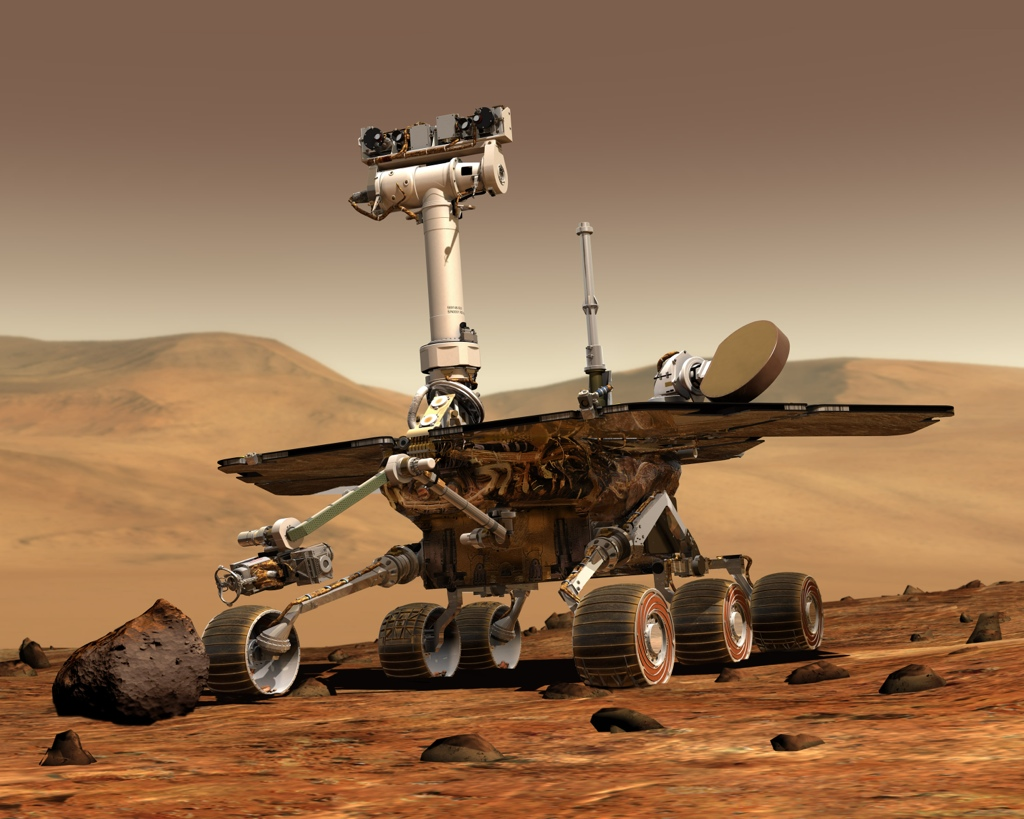
\includegraphics[width=6cm]{kapitel3/nasa_rover}
  \caption{Ein Nasa Rover}
  \label{Kap2:NasaRover}
\end{figure}


Man kann sich auch selber ein Makro für das Einfügen von Bildern schreiben:

\bild{kapitel3/modell_point_to_point}{6cm}{Point to Point}

\begin{sidewaysfigure}
 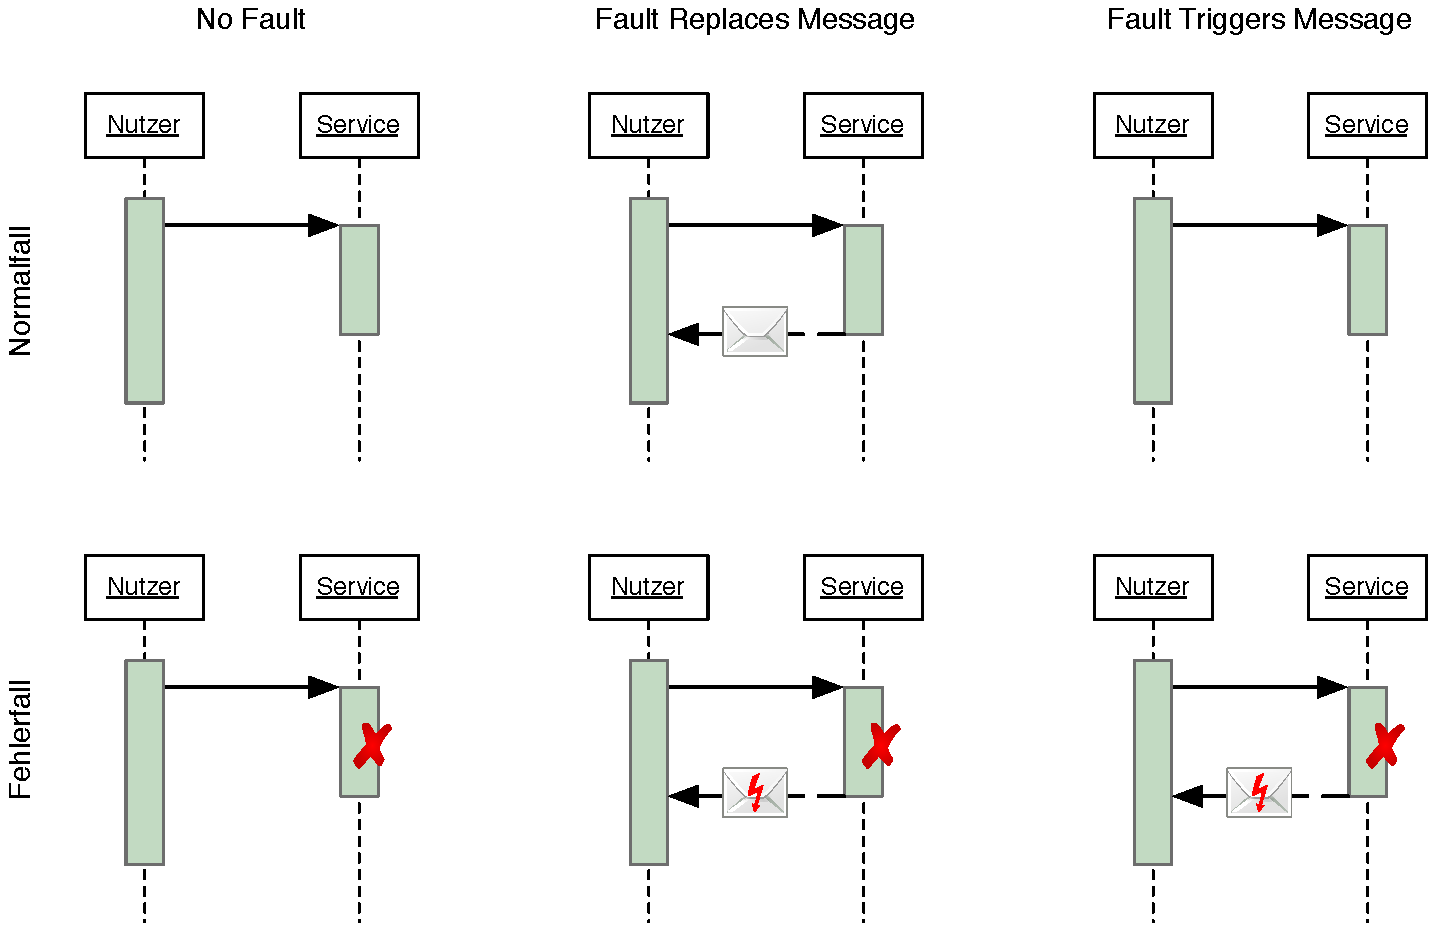
\includegraphics[width=22cm]{kapitel3/ws-wsdl20-fehler}
  \caption{Sehr große Grafiken kann man drehen, damit sie auf die Seite passen}
  \label{Kap2:wsdl-fehler}
\end{sidewaysfigure}


\clearpage % Alle Bilder, die bisher kamen ausgeben

\section{Formelsatz}

Eine Formel gefällig? Mitten im Text $a_2 = \sqrt{x^3}$ oder als eigener Absatz (siehe Formel~\ref{Formel}):

\begin{equation}
\begin{bmatrix}         
   1 &  4 &  2 \\
   4 &  0 & -3 
\end{bmatrix}        
        \cdot
\begin{bmatrix}                
   1 &  1 &  0 \\
  -2 &  3 &  5 \\
   0 &  1 &  4 
\end{bmatrix}        
       {=} 
\begin{bmatrix}               
  -7 &  15 &  28 \\
   4 &   1 & -12 
\end{bmatrix}
\label{Formel}
\end{equation}


\section{Sourcecode}

Man kann mit Latex auch ganz toll Sourcecode in den Text aufnehmen.

\subsection{Aus einer Datei}

\lstinputlisting[firstline=2,language=Java,caption={Crypter-Interface},label=lst:CrypterInterface]{\srcloc/Crypter.java}


\subsection{Inline}

\begin{lstlisting}[language=Java,caption=Methode checkKey()]
    /**
     * Testet den Schlüssel auf Korrektheit: Er muss mindestens die Länge 1
     * haben und darf nur Zeichen von A-Z enthalten.
     *
     * @param key zu testender Schlüssel
     * @throws CrypterException wenn der Schlüssel nicht OK ist.
     */
    protected void checkKey(Key key) throws CrypterException {

        // Passt die Länge?
        if (key.getKey().length == 0) {
            throw new CrypterException("Der Schlüssel muss mindestens " +
                    "ein Zeichen lang sein");
        }

        checkCharacters(key.getKey(), ALPHABET);
    }
\end{lstlisting}


\section{Anforderungen}

Anforderungen im Format des Volere-Templates (Snowcards) \autocite{Volere} können per Makro eingefügt werden.

\snowcard % Snowcard einbinden (Anpassungen in titelblatt.tex)
   {F52} % Nummer des Requirements
   {F} % Art
   {Hoch} % Priorität
   {User Authentifizierung} % Titel
   {Interview mit Abteilungsleiter} % Herkunft (Optional)
   {F12} % Konflikte (Optional)
   {Der Benutzer ist in der Lage sich über seinen
    Benutzernamen und sein Passwort am System anzumelden} % Beschreibung
   {Ein Benutzer kann sich mit seinem Firmenweiten Benutzernamen und
   Passwort über die Anmeldemaske anmelden und hat Zugriff auf die
   Funktionen des Systems} % Fit-Kriterium (Optional)
   {Benutzerhandbuch des Altsystems} % Material (Optional)

Ebenso nicht-funktionale Anforderungen mit Hilfe von Quality Attribute Scenarios. Siehe hierzu \autocite{Barbacci2003}.

\qas % Quality-Attribute Scenario einbinden (Anpassungen in titelblatt.tex)
   {NF11} % Nummer des Requirements
   {Hoch} % Priotität
   {Performance des Jahresabschlusses} % Titel
   {Endbenutzer} % Quelle
   {Startet einen Jahresabschluss} % Stimulus
   {Buchhaltungssystem} % Artefakt
   {Das System befindet sich im normalen Betriebszustand} % Umgebung
   {Jahresabschluss ist durchgeführt und kann als PDF abgerufen werden} % Antwort
   {10 Minuten} % Antwort-Maß
 % Externe Datei einbinden
% ------------------------------------------------------------------

\label{lastpage}

% Neue Seite
\cleardoublepage

% Backmatter mit normalem Zeilenabstand setzen
\singlespacing

% Römische Ziffern für die "Back-Matter", fortlaufend mit "Front-Matter"
\pagenumbering{roman}
\setcounter{page}{\value{frontmatterpage}}

% Abkürzungsverzeichnis
\chapter*{\hsmaabbreviations}
\addcontentsline{toc}{chapter}{\hsmaabbreviations}
% Tragen Sie hier alle Abkürzungen ein, die in der Arbeit benutzt werden

makeindex -s %.ist -t %.alg -o %.acr %.acn

\newacronym{abk}{ABK}{Abkürzung}
\newacronym{acm}{ACM}{Association of Computing Machinery}
\newacronym{pdf}{PDF}{Portable Document Format}
\newacronym{ieee}{IEEE}{Institute of Electrical and Electronics Engineers}
\newacronym{iso}{ISO}{International Organization for Standardization}
\newacronym[plural=ISPs,firstplural=Internet Service Providers (ISPs)]{isp}{ISP}{Internet Service Provider}
\newacronym{doi}{DOI}{Digital Object Identifier}


% Tabellenverzeichnis erzeugen
\cleardoublepage
\phantomsection
\addcontentsline{toc}{chapter}{\hsmalistoftables}
\listoftables

% Abbildungsverzeichnis erzeugen
\cleardoublepage
\phantomsection
\addcontentsline{toc}{chapter}{\hsmalistoffigures}
\listoffigures

% Listingverzeichnis erzeugen
\cleardoublepage
\phantomsection
\addcontentsline{toc}{chapter}{\hsmalistings}
\lstlistoflistings

% Literaturverzeichnis erzeugen (nach DIN)
\begin{flushleft}
\printbibliography
\end{flushleft}

% Index ausgeben
\cleardoublepage
\phantomsection
\addcontentsline{toc}{chapter}{\hsmaindex}
\printindex

\end{document}